\documentclass[a4paper,12pt,openany]{report}

\usepackage{titling}
\usepackage[margin=1in,headsep=0.5in,footskip=0.5in]{geometry}
\usepackage{graphicx}
\usepackage{float}
\usepackage{url}
\usepackage{verbatim}
\usepackage[framemethod=tikz]{mdframed}

\setlength{\parindent}{12pt}

\newcommand{\subtitle}[1]{
	\posttitle{
		\par\end{center}
		\begin{center}\large#1\end{center}
		\vskip0.5em
	}
}

\newcommand{\coverphoto}[2]{
	\postdate{
		\par\end{center}
		\begin{center}
			\includegraphics[width=15cm]{#1}
		\end{center}
	}
}

\newenvironment{wekaconsole}[1][]{

	\par \noindent
	\begin{samepage}
	\texttt{#1}
	\begin{mdframed}
	\small
	\ttfamily
}{
	\end{mdframed}
	\end{samepage}
}

\begin{document}
% title page
\title{CITS3401 Data Exploration and Mining\\
Project 2}
\subtitle{Wine Classification}
\author{Mitchell Pomery\\
21130887}
%\coverphoto{images/constructive}{XKCD 810}
\maketitle

\clearpage

% document

\section*{Introduction}
\paragraph \indent
The project specified that we are to develop several classifiers for wines using different classification methods to compare how machine learning performs compared to experts when rating different wines.
The initial data is split into two groups, red wine and white wine, available from the UCI Machine Learning Repository\cite{datasetlocation}.
Data analysis was done using Weka\cite{weka}, data mining software created by Machine Learning Group at the University of Waikato, New Zealand.
Specifically, we are using the classification and clustering tools in Weka Explorer for analysis.

\section*{Data Preprocessing}
\paragraph \indent
The initial data provided was in two files, \texttt{winequality-red.csv} and \texttt{winequality\-white.csv}, that where converted to Weka's ARFF file format using an online conversion tool\cite{csv2arff}.
This tool was used to output two datasets, dataset 1 (\texttt{ds1-red.arff} and \texttt{ds1-white.arff}) and dataset 2 (\texttt{ds2-red.arff} and \texttt{ds2-white.arff}).
Dataset 1 contains all the information that was in the original data, and is used to create the classifier.
The fields in this dataset are numeric, apart from the quality which is nominal, making it is possible to group wines that receive the same rankings in Weka.
Dataset 2 is contains all the numerical information from the original data and does not contain any information about the rankings from the wine tasters.
The aim is to cluster these so that the wines fall into groups similar to the quality attribute of dataset 1.

\section*{Clustering}
\paragraph \indent
Dataset 2 required clustering before it could be classified as the quality attribute of each data point has been removed.
Simple K means clustering was used and after experimenting, fixed acidity, volatile acidity, citric acid, and density were ignored for the red wine data.
This gave a roughly similar distribution to the qualities found in the red wine dataset.
In the white wine dataset, ignoring different combinations of attributes had very little effect on the clustering and so it did not seem possible to cluster the data points into a similar distribution to the initial data.
Comparing the clustering with the red wines quality information shows a 35\% accuracy in the groupings, while for the clustered white wines there is only 25\% accuracy.
These clusters where then outputted to \texttt{ds1-red-clustered.arff} and \texttt{ds1-white-clustered.arff} for use in classification.

\begin{wekaconsole}[Red Wine]
\begin{verbatim}
Scheme:weka.clusterers.SimpleKMeans -N 6 -A
"weka.core.EuclideanDistance -R first-last" -I 500 -S 10

Clustered Instances

0       632 ( 40%)
1       128 (  8%)
2       196 ( 12%)
3        32 (  2%)
4       339 ( 21%)
5       272 ( 17%)
\end{verbatim}
\end{wekaconsole}

\begin{wekaconsole}[White Wine]
\begin{verbatim}
Scheme:weka.clusterers.SimpleKMeans -N 7 -A
"weka.core.EuclideanDistance -R first-last" -I 500 -S 10
Clustered Instances

0      1093 ( 22%)
1       536 ( 11%)
2       832 ( 17%)
3       569 ( 12%)
4       885 ( 18%)
5       658 ( 13%)
6       325 (  7%)
\end{verbatim}
\end{wekaconsole}

\section*{Classification}

\paragraph \indent
Both dataset 1 and dataset 2 where processed by three different classifiers, naive bayes, neural networks and support vector machines.
The aim was to see how correct each classifier was and how efficiently it performed on different size inputs.
To do this, all variables, suck as test mode were kept constant.

\subsection*{Naive Bayesian}
\paragraph \indent
Naive Bayes classifiers are simple to implement, fast, and are used in real world situations such as spam filters.
They work by looking at the traits of an object, and using each individual trait to determine how likely it is that the object falls into a specific classification.
Their downside is that they assume the presence or absence of particular traits has no affect on the classification.
We used cross-validation for Naive Bayes with 10 folds in Weka to calculate classify all the wines, and compared the classifications with the quality fields.
Experimentation showed that increasing the number of folds for the red wine only had minimal effect on the accuracy of the classification.

\subsubsection*{Dataset 1}
\begin{wekaconsole}[Red Wine]
\begin{verbatim}
Scheme:weka.classifiers.bayes.NaiveBayes 
Relation:     ds1red
Instances:    1599
Attributes:   12
Test mode:10-fold cross-validation

Correctly Classified Instances         880               55.0344 %
Incorrectly Classified Instances       719               44.9656 %
Kappa statistic                          0.311 
Mean absolute error                      0.1763
Root mean squared error                  0.3198
Relative absolute error                 82.1845 %
Root relative squared error             97.7154 %
Total Number of Instances             1599
\end{verbatim}
\end{wekaconsole}

\begin{wekaconsole}[White Wine]
\begin{verbatim}
Scheme:weka.classifiers.bayes.NaiveBayes 
Relation:     ds1white
Instances:    4898
Attributes:   12
Test mode:10-fold cross-validation

Correctly Classified Instances        2168               44.263  %
Incorrectly Classified Instances      2730               55.737  %
Kappa statistic                          0.2169
Mean absolute error                      0.1721
Root mean squared error                  0.3221
Relative absolute error                 89.1485 %
Root relative squared error            103.6855 %
Total Number of Instances             4898
\end{verbatim}
\end{wekaconsole}

\subsubsection*{Dataset 2}
\begin{wekaconsole}[Red Wine]
\begin{verbatim}
Scheme:weka.classifiers.bayes.NaiveBayes 
Relation:     ds2red_clustered-weka.filters.unsupervised.attribute.Remove-R1
Instances:    1599
Attributes:   12
Test mode:10-fold cross-validation

Correctly Classified Instances        1424               89.0557 %
Incorrectly Classified Instances       175               10.9443 %
Kappa statistic                          0.8548
Mean absolute error                      0.0534
Root mean squared error                  0.1698
Relative absolute error                 21.401  %
Root relative squared error             48.0797 %
Total Number of Instances             1599     
\end{verbatim}
\end{wekaconsole}

\begin{wekaconsole}[White Wine]
\begin{verbatim}
Scheme:weka.classifiers.bayes.NaiveBayes 
Relation:   ds2white_clustered-weka.filters.unsupervised.attribute.Remove-R1
Instances:  4898
Attributes: 12
Test mode:10-fold cross-validation

Correctly Classified Instances        4267               87.1172 %
Incorrectly Classified Instances       631               12.8828 %
Kappa statistic                          0.8467
Mean absolute error                      0.0594
Root mean squared error                  0.1667
Relative absolute error                 24.7449 %
Root relative squared error             48.0952 %
Total Number of Instances             4898
\end{verbatim}
\end{wekaconsole}

\subsection*{Support Vector Machine}
\paragraph \indent
Support Vector Machine's are learning models and algorithms that analyze data and find patterns, then use the patterns for classification of data.
Unlike the Naive Bayesian classifier, the support vector machine is a non-probabilistic classifier, meaning that it will not provide uncertainty for the results.
This means that each different category needs to be separated by as large a gap as possible.

\subsubsection*{Dataset 1}
\begin{wekaconsole}[Red Wine]
\begin{verbatim}
Scheme:weka.classifiers.functions.SMO -C 1.0 -L 0.001 -P 1.0E-12 -N 0 -V -1
-W 1 -K "weka.classifiers.functions.supportVector.PolyKernel -C 250007
-E 1.0"
Relation:     ds1red
Instances:    1599
Attributes:   12
Test mode:10-fold cross-validation

Correctly Classified Instances         933               58.349  %
Incorrectly Classified Instances       666               41.651  %
Kappa statistic                          0.2905
Mean absolute error                      0.2349
Root mean squared error                  0.3301
Relative absolute error                109.5032 %
Root relative squared error            100.851  %
Total Number of Instances             1599
\end{verbatim}
\end{wekaconsole}

\begin{wekaconsole}[White Wine]
\begin{verbatim}
Scheme:weka.classifiers.functions.SMO -C 1.0 -L 0.001 -P 1.0E-12 -N 0 -V -1
-W 1 -K "weka.classifiers.functions.supportVector.PolyKernel -C 250007
-E 1.0"
Relation:     ds1white
Instances:    4898
Attributes:   12
Test mode:10-fold cross-validation

Correctly Classified Instances        2550               52.0621 %
Incorrectly Classified Instances      2348               47.9379 %
Kappa statistic                          0.1905
Mean absolute error                      0.2137
Root mean squared error                  0.3168
Relative absolute error                110.7083 %
Root relative squared error            101.9859 %
Total Number of Instances             4898     
\end{verbatim}
\end{wekaconsole}

\subsubsection*{Dataset 2}
\begin{wekaconsole}[Red Wine]
\begin{verbatim}
Scheme:weka.classifiers.functions.SMO -C 1.0 -L 0.001 -P 1.0E-12 -N 0 -V -1
-W 1 -K "weka.classifiers.functions.supportVector.PolyKernel -C 250007
-E 1.0"
Relation:     ds2red_clustered-weka.filters.unsupervised.attribute.Remove-R1
Instances:    1599
Attributes:   12
Test mode:10-fold cross-validation

Correctly Classified Instances        1506               94.1839 %
Incorrectly Classified Instances        93                5.8161 %
Kappa statistic                          0.9215
Mean absolute error                      0.2238
Root mean squared error                  0.3128
Relative absolute error                 89.7115 %
Root relative squared error             88.5878 %
Total Number of Instances             1599     
\end{verbatim}
\end{wekaconsole}

\begin{wekaconsole}[White Wine]
\begin{verbatim}
Scheme:weka.classifiers.functions.SMO -C 1.0 -L 0.001 -P 1.0E-12 -N 0 -V -1
-W 1 -K "weka.classifiers.functions.supportVector.PolyKernel -C 250007
-E 1.0"
Relation:   ds2white_clustered-weka.filters.unsupervised.attribute.Remove-R1
Instances:  4898
Attributes: 12
Test mode:10-fold cross-validation

Correctly Classified Instances        4711               96.1821 %
Incorrectly Classified Instances       187                3.8179 %
Kappa statistic                          0.9545
Mean absolute error                      0.2047
Root mean squared error                  0.3021
Relative absolute error                 85.1906 %
Root relative squared error             87.1569 %
Total Number of Instances             4898
\end{verbatim}
\end{wekaconsole}

\subsection*{Neural Network}
\paragraph \indent
Neural Networks are based off of animal's central nervous systems, by using several input sensors that transform the data before handing it on to another neuron.
The neurons are connected together in a network and work simultaneously, rather then sequentially, to process the data.
Real world applications for neural networks include speech and handwriting recognition.

\subsubsection*{Dataset 1}
\begin{wekaconsole}[Red Wine]
\begin{verbatim}
Scheme:weka.classifiers.functions.MultilayerPerceptron -L 0.3 -M 0.2 -N 500
-V 0 -S 0 -E 20 -H a
Relation:     ds1red
Instances:    1599
Attributes:   12
Test mode:10-fold cross-validation

Correctly Classified Instances         967               60.4753 %
Incorrectly Classified Instances       632               39.5247 %
Kappa statistic                          0.3585
Mean absolute error                      0.1657
Root mean squared error                  0.3021
Relative absolute error                 77.2334 %
Root relative squared error             92.3027 %
Total Number of Instances             1599
\end{verbatim}
\end{wekaconsole}

\begin{wekaconsole}[White Wine]
\begin{verbatim}
Scheme:weka.classifiers.functions.MultilayerPerceptron -L 0.3 -M 0.2 -N 500
-V 0 -S 0 -E 20 -H a
Relation:     ds1white
Instances:    4898
Attributes:   12
Test mode:10-fold cross-validation

Correctly Classified Instances        2706               55.247  %
Incorrectly Classified Instances      2192               44.753  %
Kappa statistic                          0.2839
Mean absolute error                      0.1601
Root mean squared error                  0.289 
Relative absolute error                 82.9327 %
Root relative squared error             93.0254 %
Total Number of Instances             4898     
\end{verbatim}
\end{wekaconsole}

\subsubsection*{Dataset 2}
\begin{wekaconsole}[Red Wine]
\begin{verbatim}
Scheme:weka.classifiers.functions.MultilayerPerceptron -L 0.3 -M 0.2 -N 500
-V 0 -S 0 -E 20 -H a
Relation:     ds2red_clustered-weka.filters.unsupervised.attribute.Remove-R1
Instances:    1599
Attributes:   12
Test mode:10-fold cross-validation

Correctly Classified Instances        1531               95.7473 %
Incorrectly Classified Instances        68                4.2527 %
Kappa statistic                          0.9432
Mean absolute error                      0.0183
Root mean squared error                  0.1047
Relative absolute error                  7.3361 %
Root relative squared error             29.6501 %
Total Number of Instances             1599
\end{verbatim}
\end{wekaconsole}

\begin{wekaconsole}[White Wine]
\begin{verbatim}
Scheme:weka.classifiers.functions.MultilayerPerceptron -L 0.3 -M 0.2 -N 500
-V 0 -S 0 -E 20 -H a
Relation:   ds2white_clustered-weka.filters.unsupervised.attribute.Remove-R1
Instances:  4898
Attributes: 12
Test mode:10-fold cross-validation

Correctly Classified Instances        4657               95.0796 %
Incorrectly Classified Instances       241                4.9204 %
Kappa statistic                          0.9415
Mean absolute error                      0.0195
Root mean squared error                  0.1053
Relative absolute error                  8.0972 %
Root relative squared error             30.3967 %
Total Number of Instances             4898
\end{verbatim}
\end{wekaconsole}

\section*{Results}
\paragraph \indent
The project stated that dataset 1, the unmodified dataset, and dataset 2, the clustered dataset, were to be compared through the use of classifiers.
Dataset 2 had it's classification clusters generated by an algorithmic based on scientific data, while dataset 1's classifications where assigned depending each wines sensory information.
For this reason we could assume that the classifications in dataset two will be easier to classify, as they are based off of objective data rather than subjective.
Dataset 2's results were ignored when analyzing the performance of the different classifiers.

\paragraph \indent
For dataset 1, the white wine data falls into a bell curve shape, while the majority of red wine classifications fall into two distinct bins.
This makes classification hard as there is very little variance in the data.
This difference can be seen in Figure \ref{fig:redwinedist} and Figure \ref{fig:whitewinedist}.

\paragraph \indent
The information supplied about each wine is incomplete, as it is missing attributes such as grape type, brand and cost that can effect a testers perception\cite{brandloyalty}.
Wines that sell at a higher price may be perceived as better wines, even though they contain the same physio-chemical properties as a cheaper wine.
The range of wines are limited to variants of the Portuguese "Vinho Verde" wine and the classification of the wines is subjective.
This means that for someone tasting a wine from a different region may see the same physio-chemical properties, but classify the wine completely differently.

\paragraph \indent
The neural network classifier gives the best classification rate for dataset 1, and a similar classification as the support vector machine classifier for dataset 2.
It takes a significantly for time than the support vector machine however, so for larger datasets both could be seen as valid options.
The naive Bayesian classifier gave poor results for dataset 1 as expected from it's relatively simplistic algorithms.
Across large data sets, the support vector machine is the most efficient method for classifying the data due to it's higher accuracy and low running time.


\clearpage
\section*{Figures}

\begin{figure}[ht!]
	\centering
	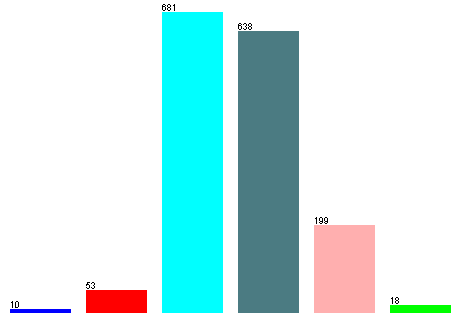
\includegraphics{images/redwinedistribution}
	\caption{Dataset 1 Red Wine Distribution}
	\label{fig:redwinedist}
\end{figure}

\begin{figure}[ht!]
	\centering
	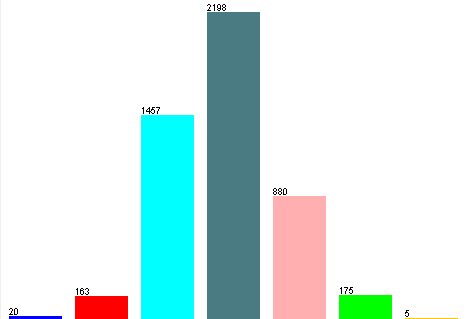
\includegraphics{images/whitewinedistribution}
	\caption{Dataset 1 White Wine Distribution}
	\label{fig:whitewinedist}
\end{figure}

\begin{thebibliography}{10}
	\bibitem{datasetlocation}UCI Machine Learning Repository: Wine Quality Data Set. 2014. UCI Machine Learning Repository: Wine Quality Data Set. [ONLINE] Available at: \url{http://archive.ics.uci.edu/ml/datasets/Wine+Quality}. [Accessed 01 June 2014].

	\bibitem{weka}Weka 3 - Data Mining with Open Source Machine Learning Software in Java . 2014. Weka 3 - Data Mining with Open Source Machine Learning Software in Java . [ONLINE] Available at: \url{http://www.cs.waikato.ac.nz/ml/weka/}. [Accessed 01 June 2014].

	\bibitem{csv2arff}Online CSV to ARFF conversion tool. 2014. Online CSV to ARFF conversion tool. [ONLINE] Available at: \url{http://slavnik.fe.uni-lj.si/markot/csv2arff/csv2arff.php}. [Accessed 01 June 2014].

	\bibitem{priorpaper}P. Cortez, A. Cerdeira, F. Almeida, T. Matos and J. Reis. Modeling wine preferences by data mining from physicochemical properties. In Decision Support Systems, Elsevier, 47(4):547-553, 2009.

	\bibitem{naivebayes}Rennie, J.; Shih, L.; Teevan, J.; Karger, D. (2003). "Tackling the poor assumptions of Naive Bayes classifiers". ICML.

	\bibitem{nonprobcalc}Non-Probabilistic Classification Methods. 2014. Non-Probabilistic Classification Methods. [ONLINE] Available at: \url{http://www.dcs.gla.ac.uk/~girolami/Machine_Learning_Module_2006/week_5/Lectures/wk_5.pdf}. [Accessed 01 June 2014].

	\bibitem{brandloyalty}Brand Loyalty: The psychology of preference | Bill Nissim | brandchannel.com. 2014. Brand Loyalty: The psychology of preference | Bill Nissim | brandchannel.com. [ONLINE] Available at: \url{http://www.brandchannel.com/papers_review.asp?sp_id=680}. [Accessed 02 June 2014].

\end{thebibliography}

\end{document}